% Chapter IV
\makeatletter
\def\input@path{{../}}
\makeatother
\documentclass[../main.tex]{subfiles}
\begin{document}
\chapter{Cloud voids - interpretation and explanation} % Chapter title

\label{ch:holes} % For referencing the chapter elsewhere, use \autoref{ch:name} 

This chapter presents experimental, theoretical and numerical results concerning cloud voids. Cloud voids are a phenomenon that was registered only once and was published for the first time in \citet{Karpinska2019} by the author of this thesis and others, including the experimental group. \ref{ch4s1} presents the experimental results in details. \ref{ch4s2} proposes the necessary conditions for cloud void formation, assuming the model exploited in \autoref{ch:single} in polydisperse particle case and verifies them in cloud-like conditions.

%----------------------------------------------------------------------------------------
\section{Cloud voids experiment results}
\label{ch4s1}
Cloud voids observations were performed at UFS on Zugspitze slopes in August 2011. Experimental methods used were described in Sec.\autoref{ch2s4}. This section presents the measurement results.\\
First, 30-minute long records of turbulence and droplet properties corresponding to the camera acquisition series in two measurement days were chosen for analysis. Droplet size raw measurements are presented in Fig. \ref{fig:ch4_1} and the corresponding statistics in Table \ref{tab:ch4_1}. Both cloud droplets, as well as drizzle drops were captured. On August 29th the droplet number concentration was visibly larger. Unfortunately the device deficiency did not allow for reliable measurement of the droplet concentration on August 29th. Next, the probability distribution of the droplet size has been calculated and presented in Fig.\ref{fig:ch4_2}. There are clear differences between the distributions measured on both days: the first one is much wider, the tail reach larger values and on average the droplets are about twice as big.

\begin{figure}[h]
\centering
\noindent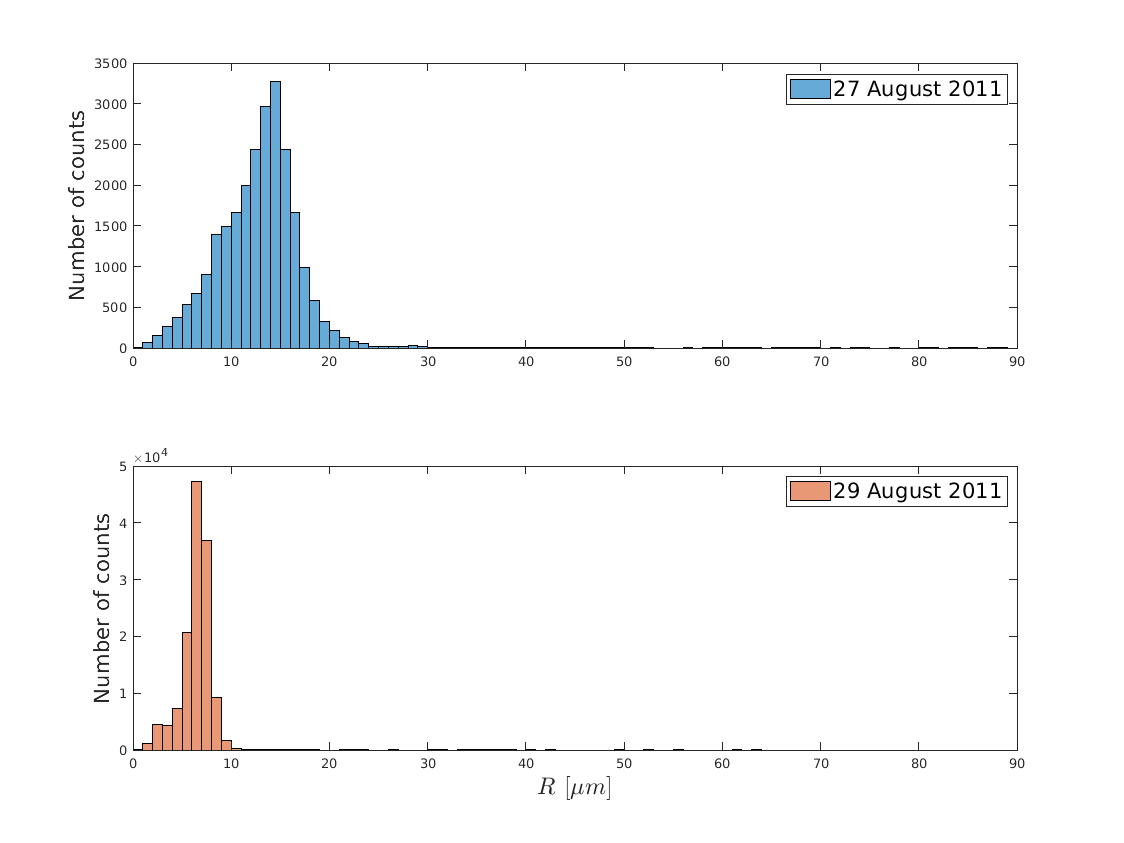
\includegraphics[width=30pc]{gfx/Hist_counts_raw.png}
\caption{Histograms of droplet size counts measured with a PDI probe at the UFS on 27th and 29th of August 2011.}
\label{fig:ch4_1}
\end{figure}

\begin{figure}[h]
\centering
\noindent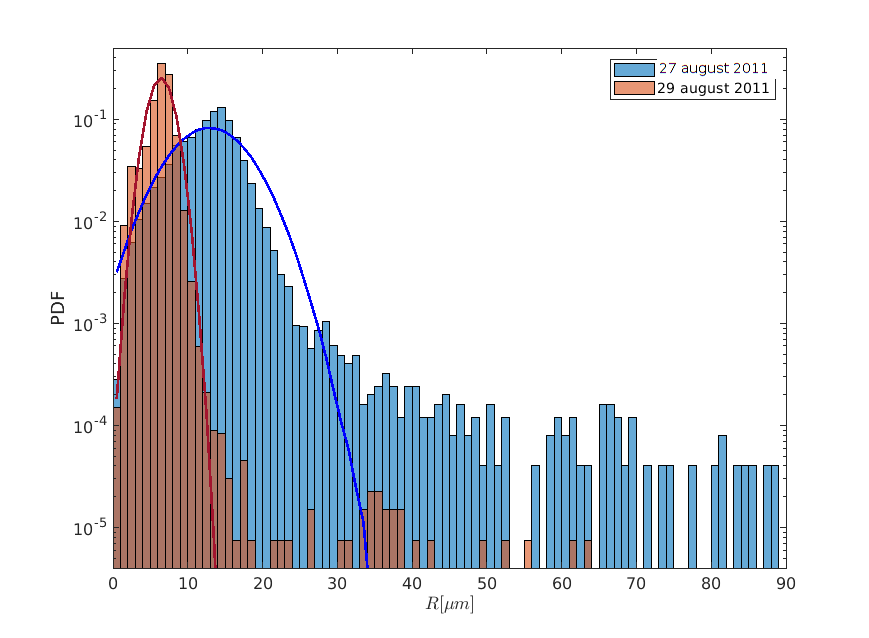
\includegraphics[width=30pc]{gfx/PDFs_log.png}
\caption{Droplet size probability distributions calculated for the data obtained with a PDI probe at the UFS on 27th and 29th of August 2011.}
\label{fig:ch4_2}
\end{figure}

High-resolution measurements of small-scale turbulence during cloud void events were conducted. Applying the methods described in Sec. \autoref{subs:atmosmeas}, mean energy dissipation rates and Kolmogorov scales were determined. Droplet and turbulence measured properties together with derived paremeters are summarized in Table \ref{tab:ch4_1}. Values of dimensionless parameters were calculated with the use of mean radius and Kolmogorov timescale. There is about one order of magnitude difference in $St$ between two cases, but the Froude numbers are comparable.

\begin{table}
\small
\tabcolsep=0.2cm
\caption{Properties of turbulence and cloud droplets during 30-minutes long observation periods. Values of dimensionless parameters are calculated with the use of mean radius.}
\centering
\begin{tabular}{|l|c|c|}
\hline
  & August 27th & August 29th\\
\hline
 Energy dissipation rate $\epsilon$ [cm$^2$/s$^3$] & 550 & 700 \\
\hline
 Kolmogorov length scale $\eta$ [mm] & 0.50  & 0.47\\
\hline
Komogorov timescale $\tau_{\eta}$ [ms] & 17 & 15\\
\hline
Droplet radius $R$ [$\mu$m] & 12.9 $\pm$ 4.8 & 6.4 $\pm$ 1.5\\
\hline
 Stokes number $St$ & 0.126  & 0.035\\
\hline
 Sedimentation parameter $S_v$ & 0.676  & 0.172\\
 \hline
 Froude number $Fr$ & 0.186  & 0.203\\
 \hline
 Number density $n$ [cm$^{-3}$] & 56 $\pm$ 47 & no data\\
 \hline
%\multicolumn{2}{l}{$^{a}$Footnote text here.}
\end{tabular}
\label{tab:ch4_1}
\end{table}

Multiple cloud images and movies were collected by laser-sheet imaging technique on the measurement days. In general two kinds of events in which droplet spatial distribution is visibly inhomogeneous were distinguished. The first kind is characterized by an irregular interface separating clear-air and cloudy-air volumes and/or cloudy volumes of visibly different properties over a wide range of spatial scales (panel b) in Fig. \ref{fig:ch4_3}). Inhomogeneities of the second kind, present within the cloudy volumes, were called cloud voids in ``Swiss cheese" clouds. Cloud voids were small (a few centimetres scale), the interface was usually blurry (see panels a) and c) in Fig. \ref{fig:ch4_3}) and the shapes of clear-air regions were often close to round or elliptic (see magnified voids in Fig. \ref{fig:ch4_4}). It is important to point out that the more intuitive expression "cloud holes" with regards to the second kind inhomogeneities is avoided on purpose because it is commonly used referring to the cloud-free regions occurring in stratocumulus decks, as described for example in \citet{Gerber_2005}.

\begin{figure}[h]
\centering
\noindent\includegraphics[width=35pc]{gfx/cloud_inhomog.png}
\caption{Examples of cloud voids observed at the UFS station with various camera-laser configurations. Images taken on 27 August (panel a) were chosen to estimate cloud void sizes. The ones recorded on 29 August evening (panel b) show the difference between inhomogeneities produced by cloud voids and those resulting from the mixing with clear air at the cloud edge. Other images from 29 August (panel c) suggest that the voids can be quite frequent in the sample volume. Bright spots and lines are due to presence of larger precipitation particles. 10~cm long segment is shown to represent spatial scale assumed in the void size calculation. For more details, see the movies attached in the supplementary materials.}
\label{fig:ch4_3}
\end{figure}

Inhomogeneities of the first kind are argued to be created in the process of cloud -- clear-air mixing (e.g. \cite{Warhaft_2000}). In contrast, in some series of images and movies, the shape of the recorded tracks of cloud droplets suggest the following cloud void origin hypothesis: they result from interactions between inertial, heavy cloud droplets and small-scale vortices present in a turbulent cloud. Comparison of the two described cases becomes straightforward when conducted on the basis of the enclosed movies \citep{database}. In the movie "ms01" between 13~s and 22~s there are two cloud void appearances. Motion of the void in the homogeneous cloud field resembles motion of a worm. Movie "ms02" presents cloudy and clear air mixing at the cloud edges. \\

\begin{figure}[h]
\centering
\noindent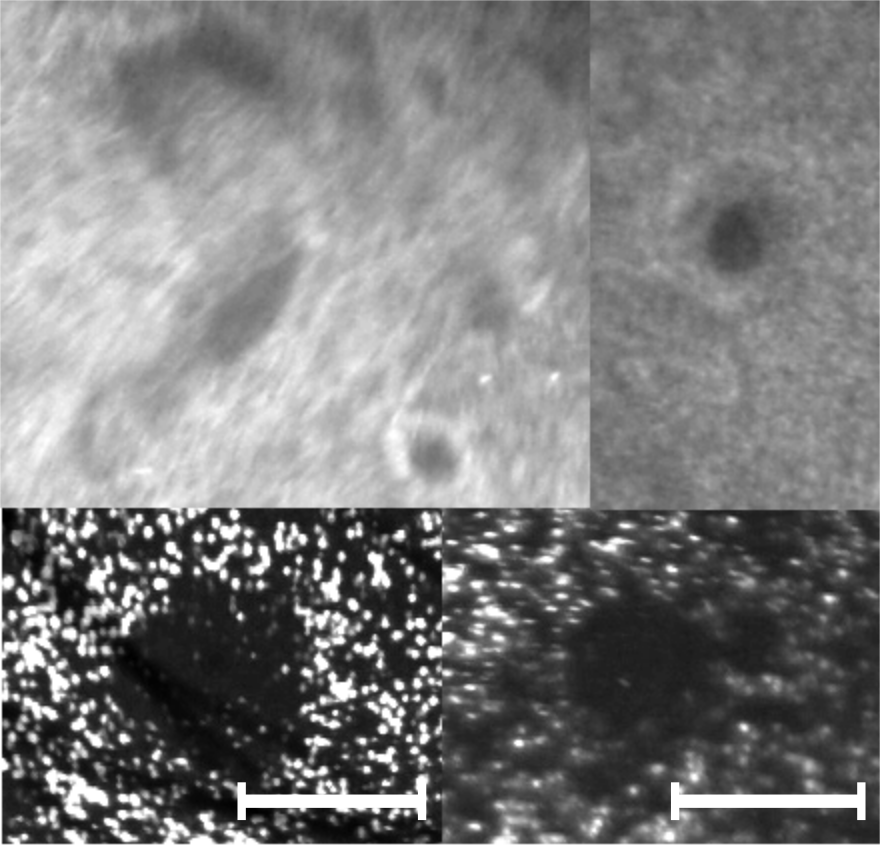
\includegraphics[width=35pc]{gfx/closeups.png}
\caption{Example close-ups of variously shaped cloud voids observed at the UFS station with different camera-laser configurations. 5~cm long section is placed in each image to represent spatial scale assumed in the void size calculation.}
\label{fig:ch4_4}
\end{figure}

There were a few series of cloud void images collected with various laser-camera settings on the two experimental days. The best quality series, made in the morning of the 27th, was chosen for void size analysis. For the series of 17 photos selected for analysis, there were four in which voids were not clear enough to be accounted for. In the remaining 13 photos 27 voids were identified. Each one's size was manually determined. In the case of a round void, the diameter was taken as the size; in a case of flattened or ellipsoidal void, the maximal chord was taken. The typical void diameter was estimated to be 3.5$\pm$1~cm; the maximal, 12$\pm$4~cm; the minimal, 1$\pm$0.5~cm. Images from the analysed series from the morning of August 27th showing examples of objects identified as voids are presented in the panel a) of Fig. \ref{fig:ch4_3}. Voids captured on the 29th of August were not analysed due to the large uncertainty resulting from the unknown geometry of the camera-laser set-up. The general experimental observation was that the voids were smaller then those on August 27th. Definitive experimental verification of the cloud void origin is not possible on the basis of collected data only; however, in next sections, I argue that void creation due to inertia of droplets present inside vortex tubes is highly probable.

%------------------------------------------------
\section{Cloud void creation conditions}
\label{ch4s2}
Lets assume that cloud voids are caused by the presence of a long-lasting vortex that appear numerously in turbulence structure and lets use the model of particle motion in a vortex explored in \autoref{ch:single}, applied to cloud particles in atmospheric turbulence. Is the model able to produce a "void effect"? If yes, what are the necessary conditions? How they translate to model parameters? This section tries to answer all these questions.\\
The use of analytical model requires the precise definition of a void. For the start, we have a collection of cloud droplets of certain size distribution, distributed uniformly in the air, where the appearance of a Burgers vortex of a certain size, circulation and gravity alignment, creates a void of a few centimetres size, lasting a few seconds. Here the void is defined as an inhomogeneity in droplet field, a region almost devoid of droplets. It has nearly cylindrical shape, in the cross section it takes a form close to a circle or an ellipsoid. In order to obtain a void using the model, the following hypothesis on polydisperse particle collective behaviour are formulated. Firstly, the majority of droplets' trajectories are determined by limit cycle attraction. Secondly, the radius of curvature of the limit cycle is large enough to recognize it, as the void in observations is clearly distinguishable from random spatial distribution fluctuations. Attraction by a single stable equilibrium point far from the axis is not considerable, so the trajectories do not cross the void. Finally, the time needed to form the void is shorter then exit time for most of the particles. These conditions are inspected in the following subsections.

\subsection{Polydisperse droplet trajectories}
\label{ssec:poly}

%Obtaining a general mathematically strict condition for creation of an arbitrary sized void in arbitrary polydisperse collection of droplets would be too detailed and too complicated to be profitable for the interpretation of crude experimental results. 
The conditions defined above for the motion of the polydisperse collection of droplets in the 2D space are met if most of the drops realize motion scenarios referred to in Fig. \autoref{fig:ch3_9} as (1b)-(3b), and possibly only a small part of the largest droplets of scenario (5). If there is a void characterized by $(A,\delta,\theta)$, then the size range $[R_<,R_>]$ of particles that realize one or more of the scenarios (1b)-(3b) is constrained. All of the particles must have at least one unstable focus $r^+_0$ near the axis. This is guaranteed by the two conditions: $r^+_0<r_s$ and $A<A_{max}(R,\delta,\theta)$ for all $R \in [R_<,R_>]$. So for a vortex described by $(A, \delta, \theta)$ the range $[R_1,R_2]$ is approximately defined by $A_{max}$ as described in last paragraph of \autoref{ch3s2ss2}. However, it can be further restricted by the condition $r^+_0<r_s$. To verify the last, a value called $R_s$ is calculated numerically and it is defined by the relation $r^+_0(R_s,A,\delta,\theta)=r_s$. Finally, limit cycle is a solution for a range of particle radii $[R_<,R_>]$ if:
\begin{itemize}
\item $R_1<R_s<R_2$, then $R_<=R_1$, $R_>=R_s$, or
\item $R_1<R_2<R_s$, then $R_<=R_1$, $R_>=R_2$.
\end{itemize}
Figure \ref{fig:ch4_5} presents results of numerical calculations of $R_1$, $R_2$, $R_s$ in the vortex parameters domain, specific for cloud-like conditions (first, second and third row respectively). Colour scale was selected to be common to all three variables. Alignment angle $\theta$ cases are arbitrary, but smaller then $\pi/4$, for the clarity of the figures. For the larger the angle, the narrower the $A$ and $\delta$ domain in which limit cycle is a solution. The fourth row shows the difference $R_2-R_s$. $R_1$ decreases when strain parameter $A$ decreases (circulation increases) or vortex size $\delta$ decreases. On the contrary to $R_1$, $R_2$ and $R_s$ increase when strain parameter $A$ decreases (circulation increases) or vortex size $\delta$ decreases. The last row reveals, that the inequality sign between $R_2$ and $R_s$ is not constant, but changes with vortex parameters. $R_>$ should be calculated in two ways, depending on these parameters.

\begin{figure}[h]
\centering
\noindent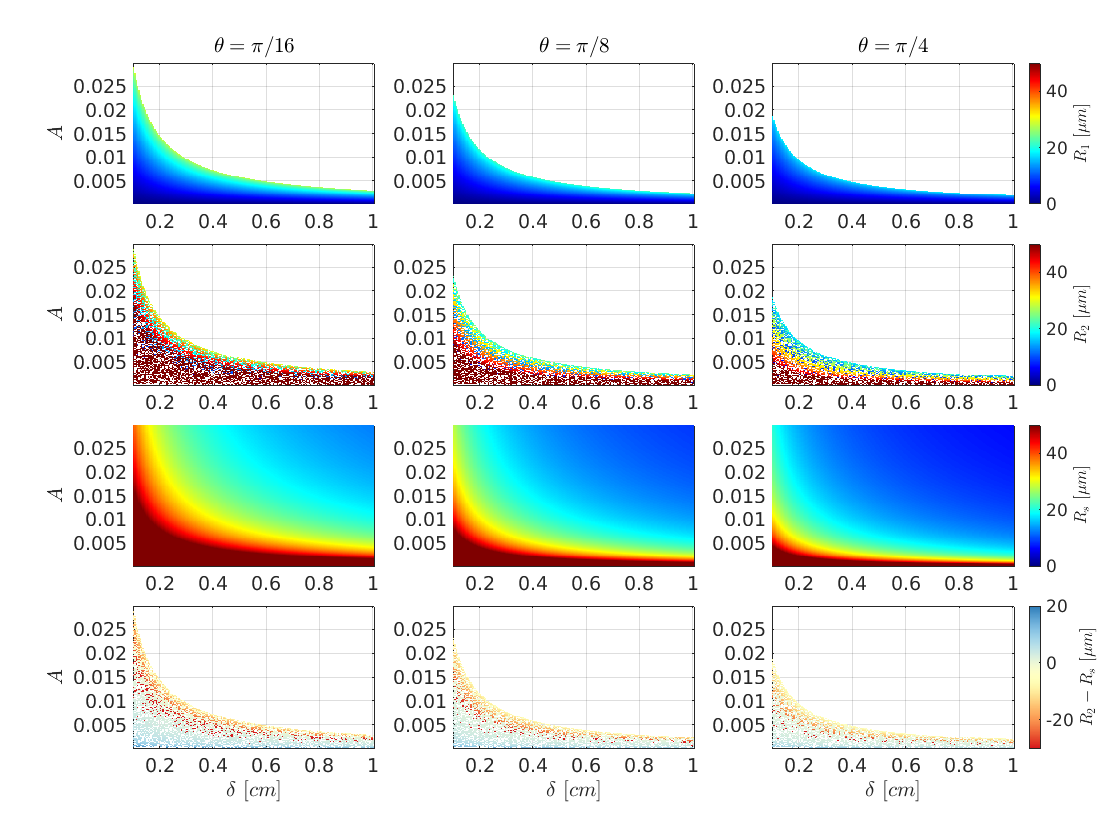
\includegraphics[width=35pc]{gfx/R1R2Rs.png}
\caption{Approximated size range of particles $[R_1,R_2]$ that has a limit cycle solution, represented by color scale, with respect to vortex parameters (first and second row), $R_s$ (third row), as defined in the text body and the interval between $R_2$ and $R_s$ (fourth row), obtained numerically. Colorscale is common for $R_1$, $R_2$ and $R_s$, separate for $R_2-R_s$. Three alignment angle values selected are represented in columns. Vortex parameters domain corresponds to cloud-like conditions.}
\label{fig:ch4_5}
\end{figure}

Figure \ref{fig:ch4_5} shows final results: left margin of the range $R_>$, right margin of the range $R_<$ and their interval magnitude, thus giving approximate parameter ranges of cloud void-creating vortex. Colour scales in this case differ to highlight the accurate values. Presented $R_<$ values reach from around 29~$\mu m$ for $\theta=\pi/16$ and around 19~$\mu m$ for $\theta=\pi/4$ to well below 1~$\mu m$, so they are surely relevant for cloud droplets. $R_>$ has opposite $A$ dependence and it reaches from around 17~$\mu m$ for all three $theta$ to particle sizes that are far out of cloud droplets bounds. What is interesting, is the interval magnitude $\Delta R$. The minimal value of those presented in the figure is $min(\Delta R)=27, 14, 4 \ \mu m$ for $\theta=\pi/16, \pi/8, \pi/4$ respectively. These are also values that are of the same order as in cloud conditions.

\begin{figure}[h]
\centering
\noindent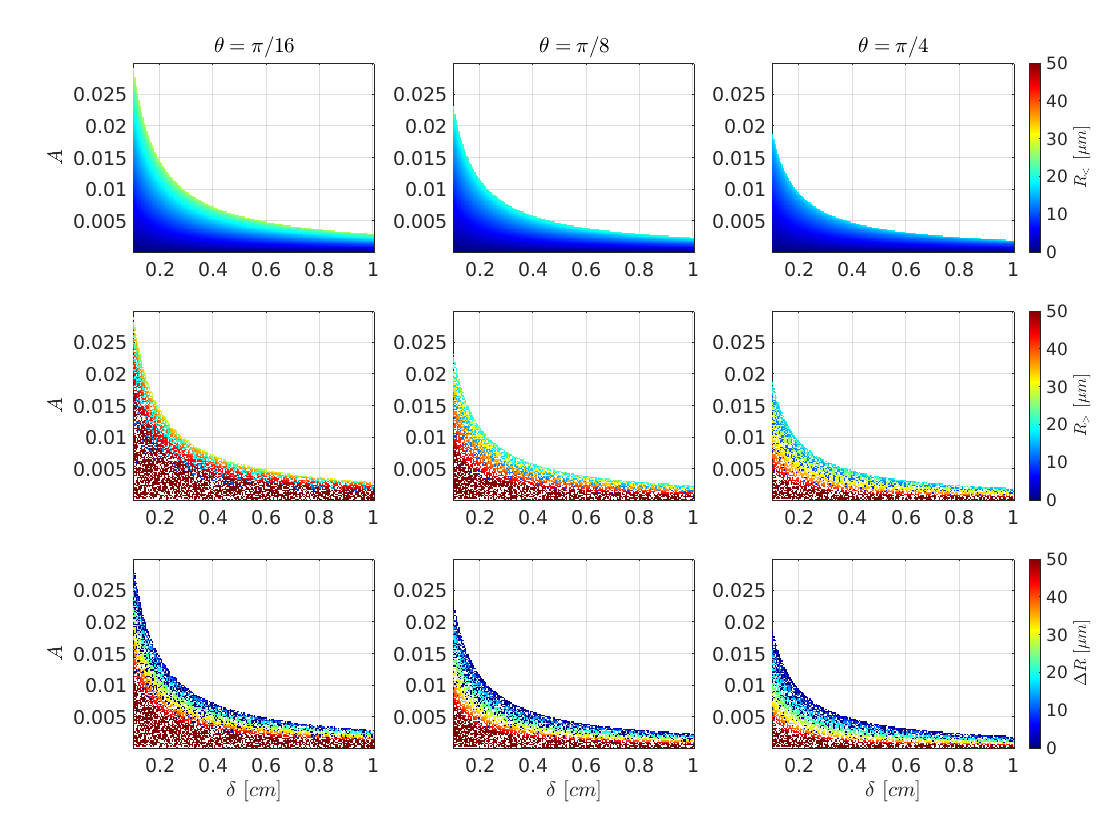
\includegraphics[width=35pc]{gfx/RlRrDeltaR.png}
\caption{Numerical calculation of approximated size range of particles $[R_<,R_>]$ (first and second row) that create a cloud void, as well as interval between them $\Delta R$ (third row) in relation with vortex parameters. Colorscale is common for $R_>$ and $\Delta R$. Three alignment angle values selected are represented in columns. Vortex parameters domain corresponds to cloud-like conditions.}
\label{fig:ch4_6}
\end{figure}

$R_1$ decreases when strain parameter $A$ decreases (circulation increases) or vortex size $\delta$ decreases. On the contrary to $R_1$, $R_2$ and $R_s$ increase when strain parameter $A$ decreases (circulation increases) or vortex size $\delta$ decreases.

Finally some general clues about cloud void formation in 2D on the basis of theoretical model are lined:
\begin{enumerate}
\item There is a threshold (minimal) value of circulation needed for void creation (corresponding to $A_{max}$. It increases with inclination angle ($\sin \theta$) and vortex size $\delta$.\\
\item The greater the circulation the smaller particles have their unstable points near the axis.
\item The range of particles having unstable points near the axis increases with increasing circulation and decreases with increasing inclination angle and vortex size $\delta$.
\end{enumerate}

\noindent Building up on these results it may be concluded that theoretical void formation conditions can be fulfilled in cloud-like conditions when it comes to 2D space. According to the model it should be harder to observe voids in vortices of larger $\delta$. When it comes to the inclination, the larger the angle, the smaller the particles thrown out of vortex center. On the other hand, increasing inclination angle decreases the range of particles circling around the void. However, larger droplets motion resemble then sedimentation through the vortex and altogether increasing inclination angle might facilitate void formation. The last conclusion is that it should be more difficult to observe voids the larger particle size range is.\\

\subsection{Void size estimation}
\label{ssec:par}
The curvature of droplet trajectories should be large enough for a void to be noticeable. In order to estimate the curvature radius we perform the following reasoning. In the face of lack of analytical limit cycle solution, droplet trajectory curvature radius can be approximated by the periodic orbit radius, which was explored in detail in \autoref{ch3s2ss1sss1}. For this reason, stable periodic orbit radius numerical calculation results are presented in a novel form in Fig.\ref{fig:ch4_30} for various representative vortex parameters. Every color represents one of droplet sizes: $R=3,13,23$~$\mu m$ chosen to be within the experimental range for August 27th (see Table \ref{tab:ch4_1}). The figure illustrates contour plots for selected orbit radii (0.5~cm ,2~cm, 5~cm), corresponding to cloud void sizes observed. Overlapping (blue on a top, then pink and green) coloured surfaces match subspaces of stable periodic orbit existence. 

Figure \ref{fig:ch4_30} shows the results of $r_{orb}$ calculation in a different view. 
\begin{figure*}
\centering
\noindent 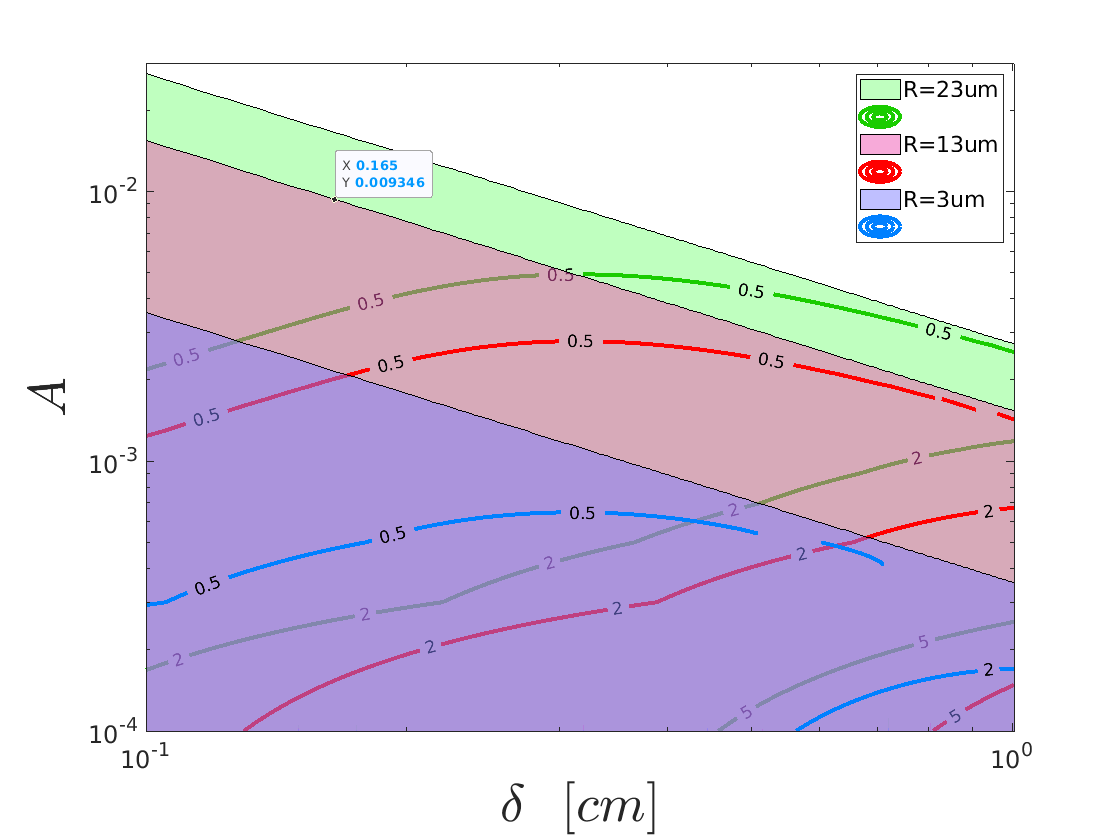
\includegraphics[width=30pc]{gfx/void_radii_R_3_13_23.png}
\caption{Contour plot of stable periodic orbit radius for droplets of radii $R=3,13,23 \ \mu m$ for cloud-like parameter ranges of $\delta$ and $A$. Overlapping (blue on a top, then pink and green) coloured surfaces match parameter domains in which stable periodic 2D orbit exist for droplet radius given by its colour. Dashed lines are contour plots for $r_{orb}$ equal to 0.5~cm ,2~cm, 5~cm. Black points represent simulation parameters sets (filled later, referred to in ???).}
\label{fig:ch4_7}
\end{figure*}

Figure \ref{fig:ch4_7} further narrows down the void-forming parameter domain.

\subsection{Timescales of motion}
Timescales of motion found for a single particle can be interpreted in the case of polydisperse collection of particles. Lets take the arbitrary range of sizes $[R_<,R_>]$ and find the relations between their timescales. Firstly, motion along vortex axis is governed by $\tau_z$ quantity, which approximately does not depend on particle size. Difference in total exit times results from the difference of equilibrium point position $z_b \propto R^2$ and according to Eq.\ref{ch3:eq14}:
\begin{equation}
\frac{\tau_{ex >}}{\tau_{ex <}}=\frac{log(L(Z^*_>,z_{0 >}^*)}{L(Z^*_<,z_{0 <}^*)}.
\label{ch4:eq1}
\end{equation}
When it comes to circular orbit timescale, there is:
\begin{equation}
\frac{\tau_{orb >}}{\tau_{orb <}}=\frac{R_>}{R_<},
\label{ch4:eq2}
\end{equation}
so it increases proportionally with droplet size. Finally the relations for docking times are implicit. Figure \autoref{fig:ch3_4b} - tu opisac, ze tam gdzie dazy do nieskonczonosci czas dokowania, to wiadomo, ze szybciej wypadna przez tau_z mniejsze. A takie regiony sa dwa. Moze ten wykres przerobic na delta i A, zeby byl porownywalny z tymi powyzej?
\section{Summary}
3D void formation due to the presence of Burgers vortex in droplets field is fully possible for cloud-like conditions.
%------------------------------------------------

\end{document}